\textit{Solución.} A partir de los \hyperref[eq3]{parámetros del modelo linealizado} y los datos del \hyperref[t1]{Cuadro 1}, se obtienen sus valores numéricos a continuación:

\begin{alignat*}{2}
    T &= \frac{2A}{X _{vs0} K _{vs}} \sqrt{ \frac{H_0}{\rho g}} &&= \SI{315.0506}{s}\\
    K _{1} &= \frac{2}{X _{vs0} K _{vs}} \sqrt{ \frac{H_0}{\rho g}} &&= \SI{63.0101}{\second\per\metre\squared}\\
    K _{2} &= - \frac{2 H_0}{X _{vs0}} &&= \SI{-10}{m}
\end{alignat*}

\newpage

Se implementó el siguiente diagrama de bloques en Simulink.

\begin{figure}[!h]
    \centering
    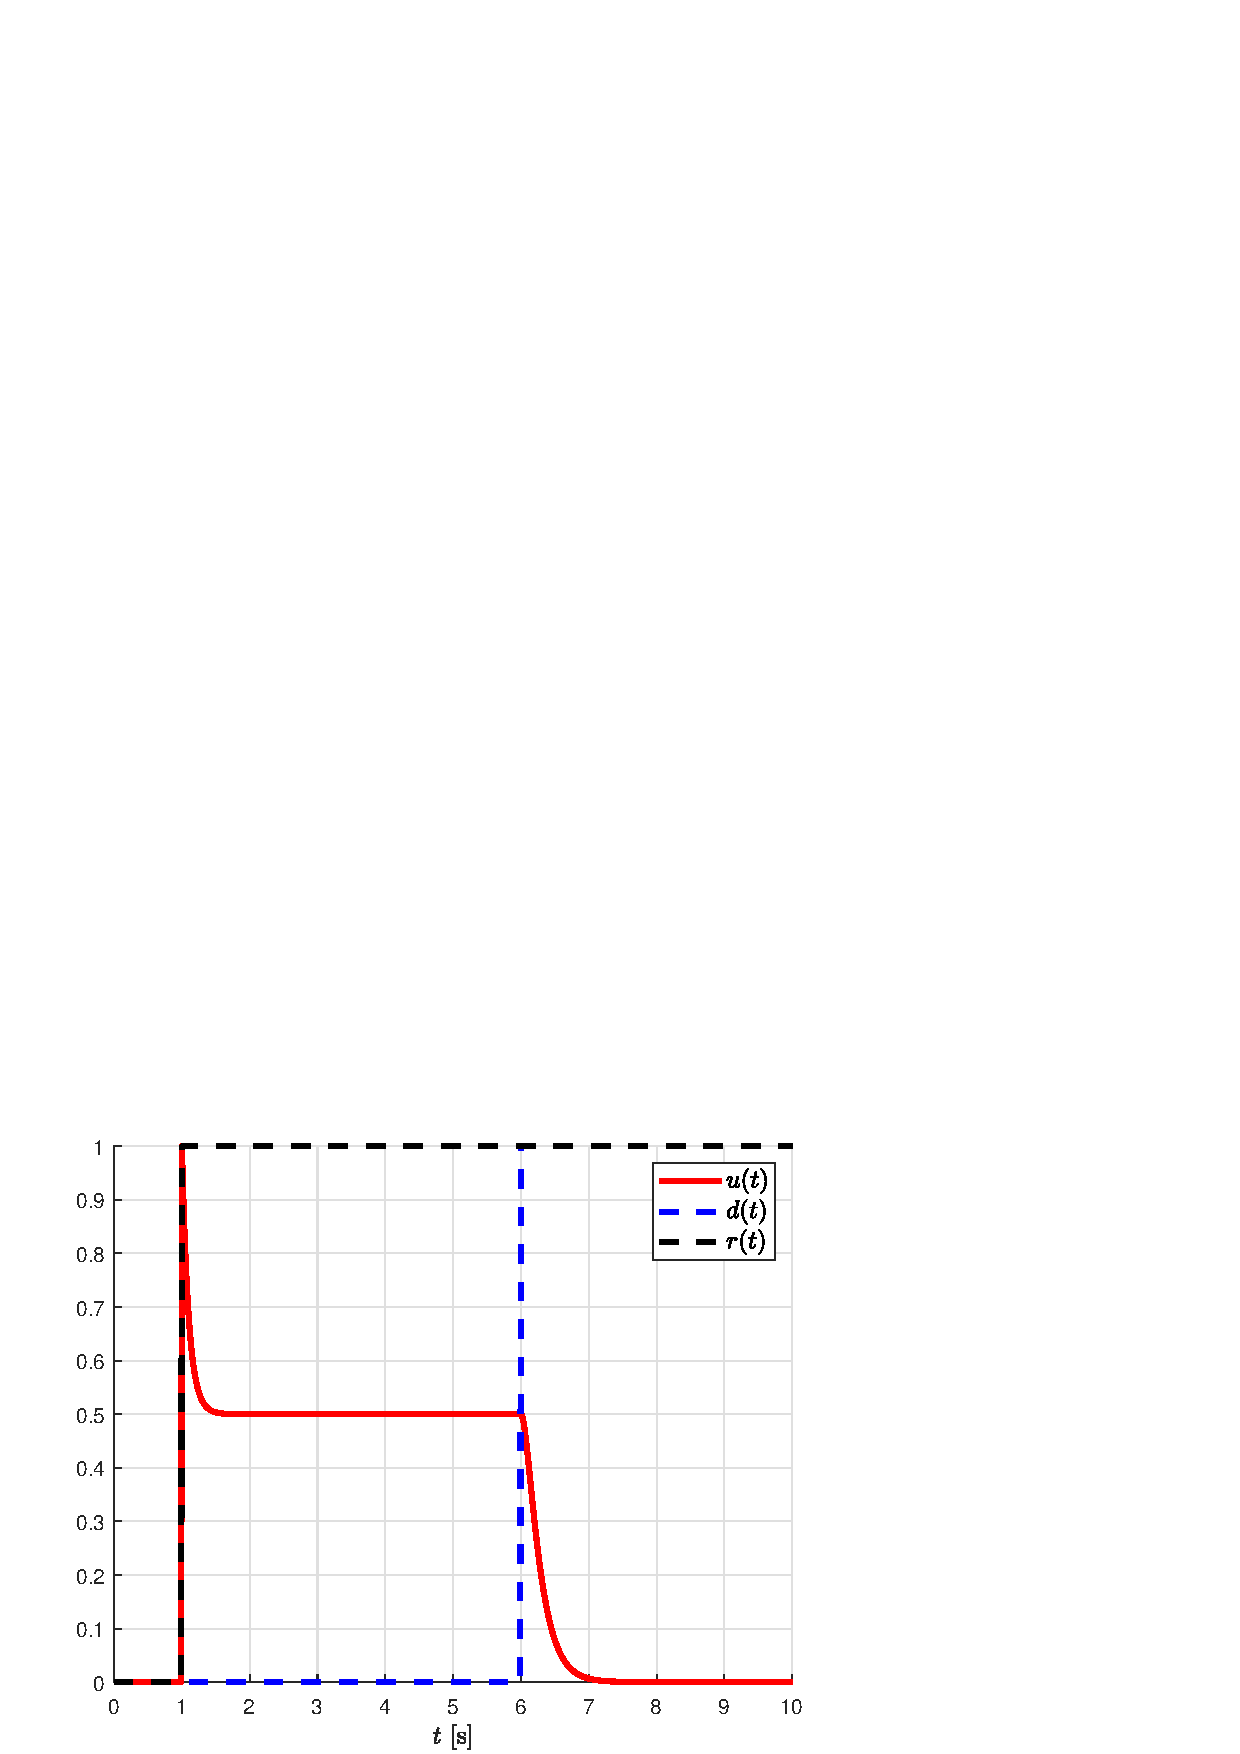
\includegraphics[width = 0.6\linewidth]{figs/fig3.png}
    \caption{Diagrama de bloques del sistema real y linealizado}
    \label{fig3}
\end{figure}
